\documentclass[titlepage,landscape]{seminar}
\usepackage{url}
\usepackage{graphicx}
\usepackage[pdftex]{color}
\usepackage{hyperref}
\usepackage{epstopdf}
\usepackage{slides}

\newcommand{\frack}{\frac{1}{k}}
\newcommand{\quarter}{\frac{1}{4}}

\begin{document}

\myslide{
\heading{Loss of beneficial alleles}
\begin{center}
\begin{tabular}{ccc}
$A_1A_1$ & $A_1A_2$      & $A_2A_2$ \\
1 + s    & $1 + \half s$ & 1
\end{tabular}
\end{center}
\vfill
}

\myslide{
\heading{Loss of beneficial alleles}
\begin{center}
\begin{tabular}{ccc}
$A_1A_1$ & $A_1A_2$      & $A_2A_2$ \\
1 + s    & $1 + \half s$ & 1
\end{tabular}
\end{center}
\vfill
\[
P_1(p) = \frac{1 - e^{-2N_esp}}{1 - e^{-2N_es}}
\]
}

\myslide{
\heading{Loss of newly arisen beneifical allele}
\begin{eqnarray*}
p &=& \frac{1}{2N} \\
P_1(p) &=& \frac{1 - e^{-2N_es(1/2N)}}{1 - e^{-2N_es}} \\
       &\approx& 1 - e^{-N_es(1/N)} \hbox{ if $2N_es$ is ``large''} \\
       &=& 1 - e^{s\left(\frac{N_e}{N}\right)} \\
       &\approx& s\left(\frac{N_e}{N}\right)
                 \hbox{ if $s$ is ``small.''}
\end{eqnarray*}
}

\myslide{
\heading{Fixation of detrimental alleles}
\begin{center}
\begin{tabular}{ccc}
$A_1A_1$ & $A_1A_2$      & $A_2A_2$ \\
1 - s    & $1 - \half s$ & 1
\end{tabular}
\end{center}
\vfill
\[
P_1(p) = \frac{1 - e^{2N_esp}}{1 - e^{2N_es}}
\]
}

\myslide{
\heading{Fixation of detrimental alleles}
\[
P_1(p) = \frac{1 - e^{2N_esp}}{1 - e^{2N_es}}
\]
\vfill
\begin{eqnarray*}
\hbox{Fixation probability of neutral allele} &=& \frac{1}{2(100)} \\
&=& 5 \times 10^{-3}
\end{eqnarray*}
\vfill
\begin{center}
\begin{tabular}{l|cc}
\hline\hline
      & \multicolumn{2}{c}{$N_e$} \\
$s$   & 4                  & 100 \\
\hline
0.001 & $4.9 \times 10^{-3}$ & $4.5 \times 10^{-3}$ \\
0.01  & $4.8 \times 10^{-3}$ & $1.5 \times 10^{-3}$ \\
0.1   & $3.2 \times 10^{-3}$ & $2.2 \times 10^{-10}$ \\
\hline
\end{tabular}
\end{center}
}

\myslide{
\heading{Genetic drift and heterozygote advantage}
\begin{itemize}

\item Genetic drift leads to the loss of genetic diversity over time. 

\item Heterozygote advantage leads to the preservation of genetic diversity.

\end{itemize}

{\color{red}\bf BUT} Heterozygote advantage may promote loss of diversity.

\begin{itemize}

\item If an allele is relatively rare, drift will tend to dominate the
  dynamics of allele frequency change, even if it's under selection.

\item If selection is ``pushing'' an allele to a relatively extreme
  frequency, it will get to the region where drift dominates the
  dynamics more rapidly than it would under drift alone.

\item So heterozygote advantage in which the two homozygotes have very
  asymmetrical fitnesses is likely to increase the rate at which
  diversity is lost. As a corollary, the allele in the disfavored
  homozygote is the most likely to be lost.

\end{itemize}
}

\myslide{
\heading{Genetic drift and heterozygote advanatage}
\begin{center}
\resizebox{!}{0.9\textheight}{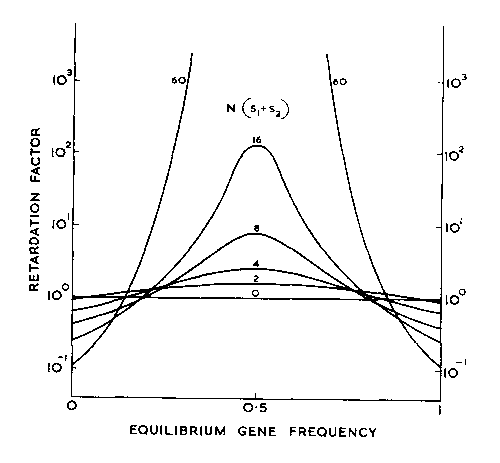
\includegraphics{drift-heterozygote-advantage.eps}}
\end{center}
}

\myslide{
\heading{Genetic draft}
\begin{center}
\resizebox{!}{0.9\textheight}{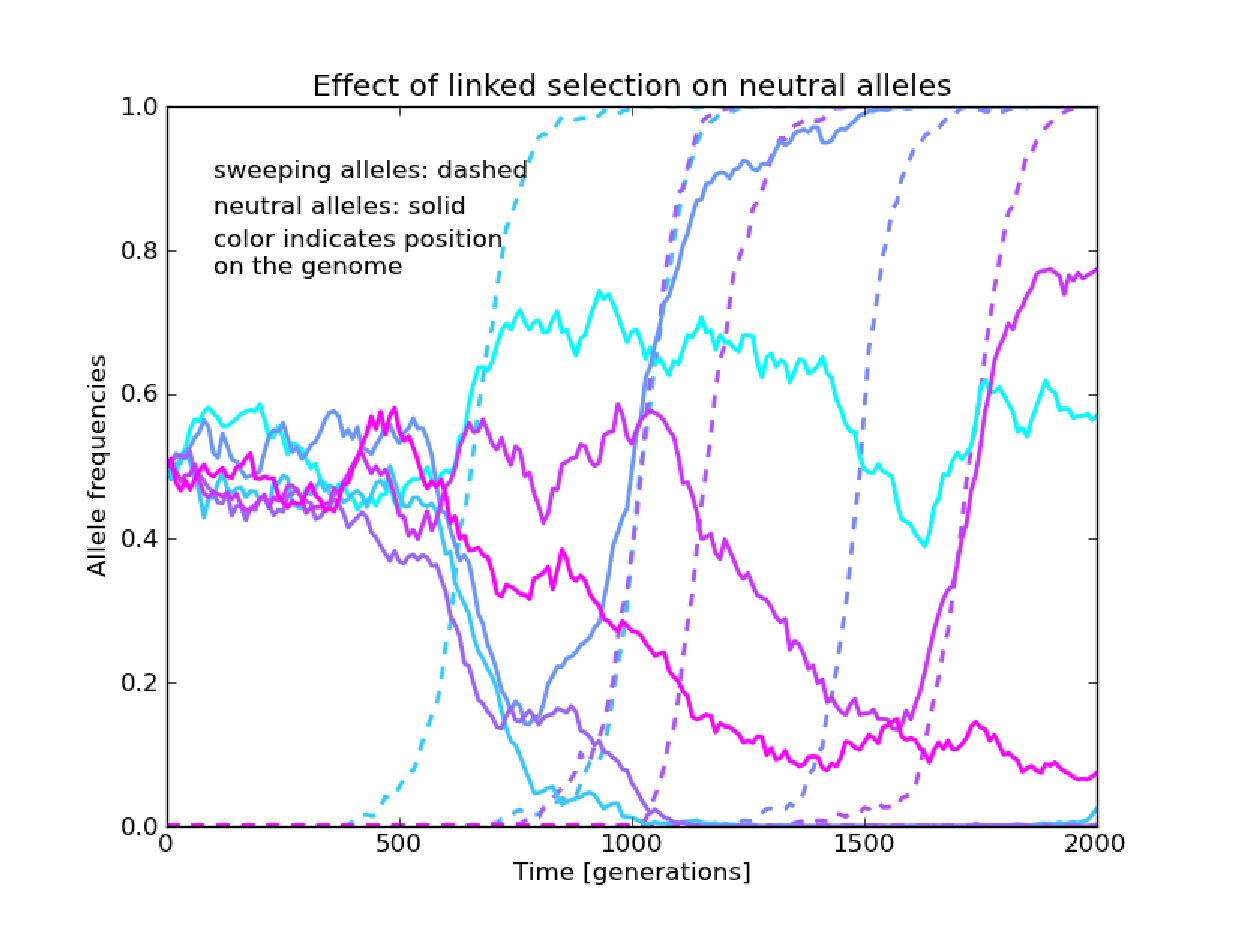
\includegraphics{genetic-draft.eps}}
\end{center}
}

\end{document}

